\documentclass[conference]{IEEEtran}
\IEEEoverridecommandlockouts
% The preceding line is only needed to identify funding in the first footnote. If that is unneeded, please comment it out.
\usepackage{cite}
%\usepackage[noadjust]{cite}  
\usepackage{amsmath,amssymb,amsfonts , nccmath}
\usepackage{algorithmic}
\usepackage{graphicx}
\usepackage{mathtools}

\usepackage{caption}
\usepackage{subcaption}
\usepackage{pgf-pie}  
\usepackage{textcomp}
\usepackage{xcolor}
\usepackage{multirow}
\usepackage{booktabs}




\def\BibTeX{{\rm B\kern-.05em{\sc i\kern-.025em b}\kern-.08em
    T\kern-.1667em\lower.7ex\hbox{E}\kern-.125emX}}
    
    

    
    
    
\begin{document}

\title{Texture Classification in Interstitial lung disease patients using Graph Signal Processing}

\author{\IEEEauthorblockN{1\textsuperscript{st} Given Name Surname}
\IEEEauthorblockA{\textit{dept. name of organization (of Aff.)} \\
\textit{name of organization (of Aff.)}\\
Tehran, Iran \\
email address or ORCID}
\and
\IEEEauthorblockN{2\textsuperscript{nd} Given Name Surname}
\IEEEauthorblockA{\textit{dept. name of organization (of Aff.)} \\
\textit{name of organization (of Aff.)}\\
Tehran, Iran \\
email address or ORCID}
\and
\IEEEauthorblockN{3\textsuperscript{rd} Given Name Surname}
\IEEEauthorblockA{\textit{dept. name of organization (of Aff.)} \\
\textit{name of organization (of Aff.)}\\
Tehran, Iran \\
email address or ORCID}
\and

%\IEEEauthorblockN{4\textsuperscript{rd} Given Name Surname}
%\IEEEauthorblockA{\textit{dept. name of organization (of Aff.)} \\
%\textit{name of organization (of Aff.)}\\
%Lausanne, Switzerland \\
%email address or ORCID}
%\and
}

\maketitle

\begin{abstract}
\end{abstract}

\begin{IEEEkeywords}
\end{IEEEkeywords}

\section{Introduction}
\vspace{0.5cm}

\section{Related work}
\vspace{0.5cm}


\section{Method}
\subsection{\textbf{Graph wavelet filter banks}}

Wavelet filter banks are among the most popular methods for extracting features from images or textures. One of their variations is graph wavelet filter banks that take into account the relation of different pixels in the texture. In this work, we used the method proposed by Qiao et al. at \cite{wavelet}. We used two-level decomposition for graph wavelet filters; after calculating the filter response with meyer kernel on the texture as discussed in \cite{wavelet}, we moved a $4\times4$ window with the stride of 1 on the response of wavelet and for each window we applied singular value decomposition. $F_1 , F_2, F_3$ sets as discussed in \cite{wavelet} are

\begin{equation}
\begin{multlined}
F_1=\{ max(S_1),max(S_2),...,\\max(S_i),...,max(S_N)\}\\
F_2=\{ mean(S_1),mean(S_2),...,\\mean(S_i),...,mean(S_N)\}\\
F_3=\{ median(S_1),median(S_2),...,\\median(S_i),...,median(S_N)\}
\end{multlined}
\end{equation}

After fitting a Weibull distribution to each set, we will get two parameters, scale and shape parameters.

For each texture, we have two level graph wavelets, and every wavelet has four subbands, every subband results in three $F_i$ sets, which will result in two parameters for Weibull distribution. Finally, we have a 48-dimensional feature vector for each texture.



Figure \ref{fig:weibull_fit} shows an example of weibull distribution fitting to $F_1$ and $F_2$ sets.
\begin{figure}[tbh]
    \centering
    \begin{subfigure}{0.24\textwidth}
        \centering
        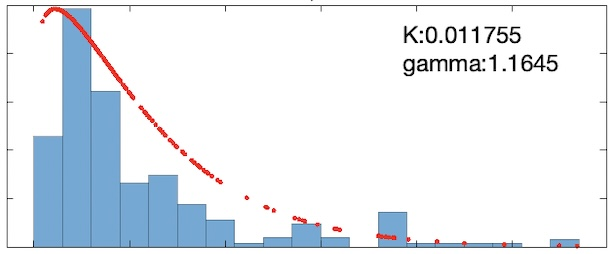
\includegraphics[width=\linewidth]{weibull1.jpg}
       \caption{}
    \end{subfigure}
    \hfill
    \begin{subfigure}{0.24\textwidth}
        \centering
        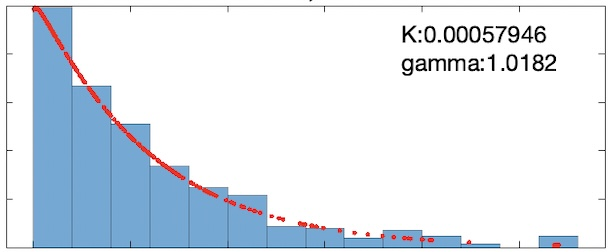
\includegraphics[width=\linewidth]{weibull2.jpg}
        \caption{}
    \end{subfigure}
    \caption{Example of Weibull fitting to $F_i$ sets}
    \label{fig:weibull_fit}
\end{figure}



%Qiao et al. at \cite{wavelet} in Figure \ref{fig:waveletsum} are showing the summary of graph wavelet method for extracting features from tesxtures.
%\begin{figure*}[tbh]
%  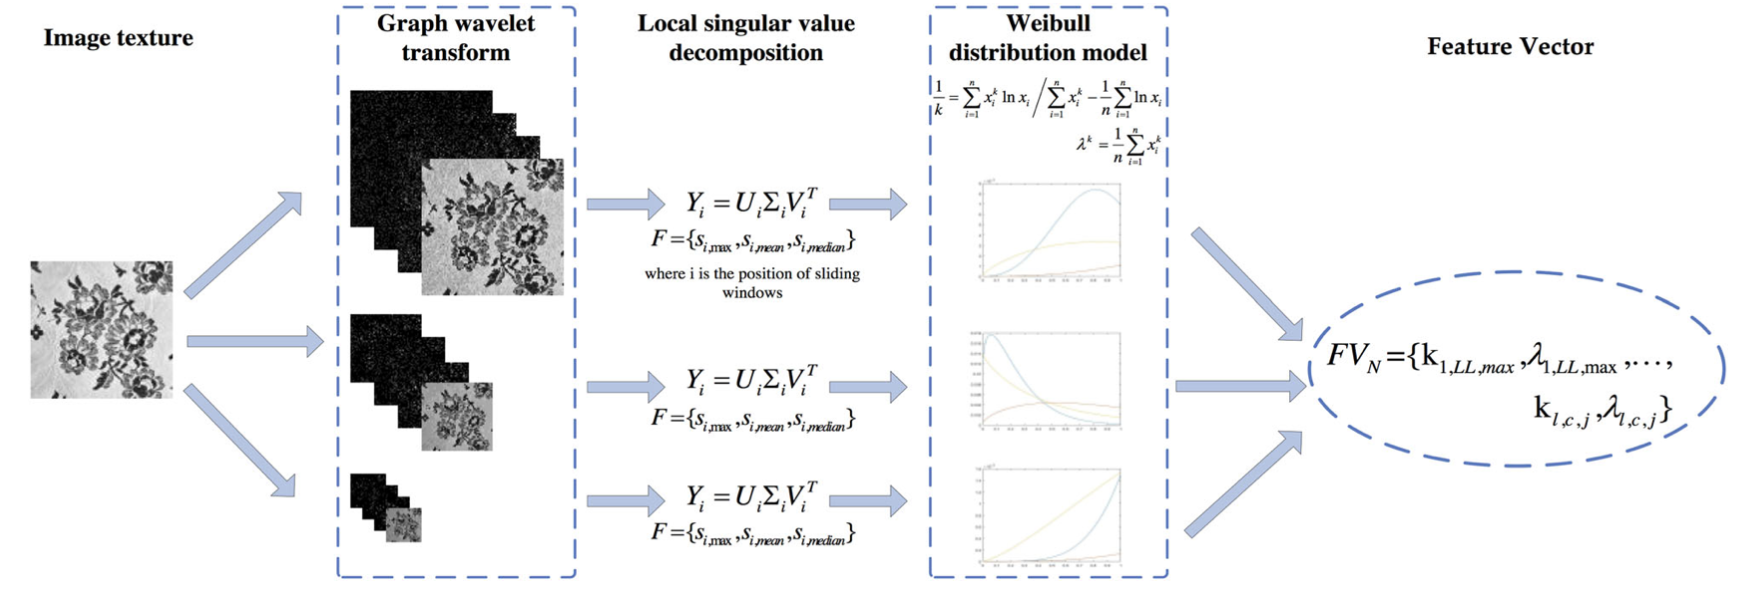
\includegraphics[width=1\linewidth]{waveletsum.png}
%      \caption{the graph wavelet method proposed in \cite{wavelet}}
%  \label{fig:waveletsum}
%\end{figure*}
%
%









\subsection{\textbf{Visibility Graphs}}
In recent yeast, increasing the popularity of complex systems and networks motivates researchers to develop methods for transforming classic signals into graph signals which help indicate the relation of signal values. one of these methods is called visibility graphs which are introduced in \cite{VG}. This method proposed in that paper is mainly applied to 1D signals. However, the concept is the same for higher dimension signals. As we know, images are 2D signals, and Iacovacci et al. in \cite{IVG} proposed a new version of visibility graphs for images called image visibility graphs.



\subsubsection{Natural Visibility Graphs}
We can connect the visibility line between two nodes with any slope in this definition. Instead, we can only have horizontal visibility lines in the horizontal visibility graph.
for the time series signal $S(t)=\{x_1,x_2,x_3,...,x_N\}$, we can define a N node natural visibility graph (N is the numbet of signal points) which $x_i$ and $x_j$ are connected only if we can find a line from $x_i$ to $x_j$ without intercepting other signal values.Equivalently $x_i$ and $x_j$ are connected if following constraint is hold,
\begin{equation}
x_k < x_i +\frac{k-i}{j-i}(x_j-x_i), \forall(i<k<j)
\end{equation}



\subsubsection{Horizontal Visibility Graphs}

The definition of horizontal visibility graphs is the same as natural visibility graphs, but we are only allowed to have horizontal lines instead of any slope for visibility lines. The  Following equation depicts this definition,
\begin{equation}
x_k < inf(x_i, x_j), \forall(i<k<j)
\end{equation}

Pei et al. in \cite{china_HVG} brough an example of HVG and NVG for a time series signal which is shown in Figure \ref{fig:VG_example}


\begin{figure}[tbh]
    \centering
    \begin{subfigure}{0.45\textwidth}
        \centering
        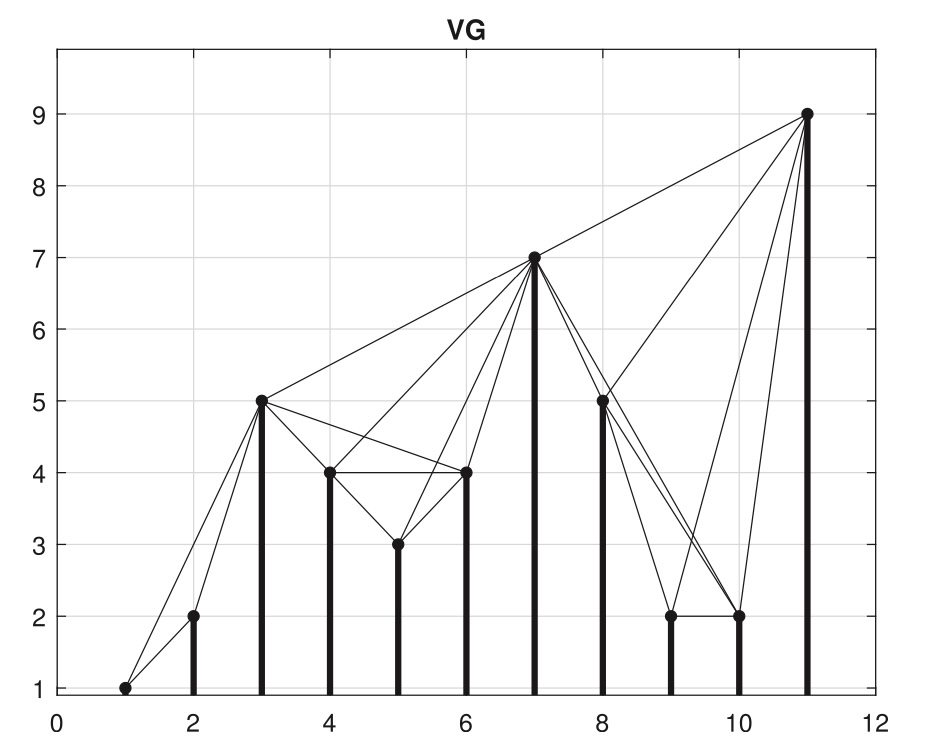
\includegraphics[width=\linewidth]{NVG.jpg}
        \caption{Natural visibility graph}
        \label{fig:NVG_example}
    \end{subfigure}
    \hfill
    \begin{subfigure}{0.45\textwidth}
        \centering
        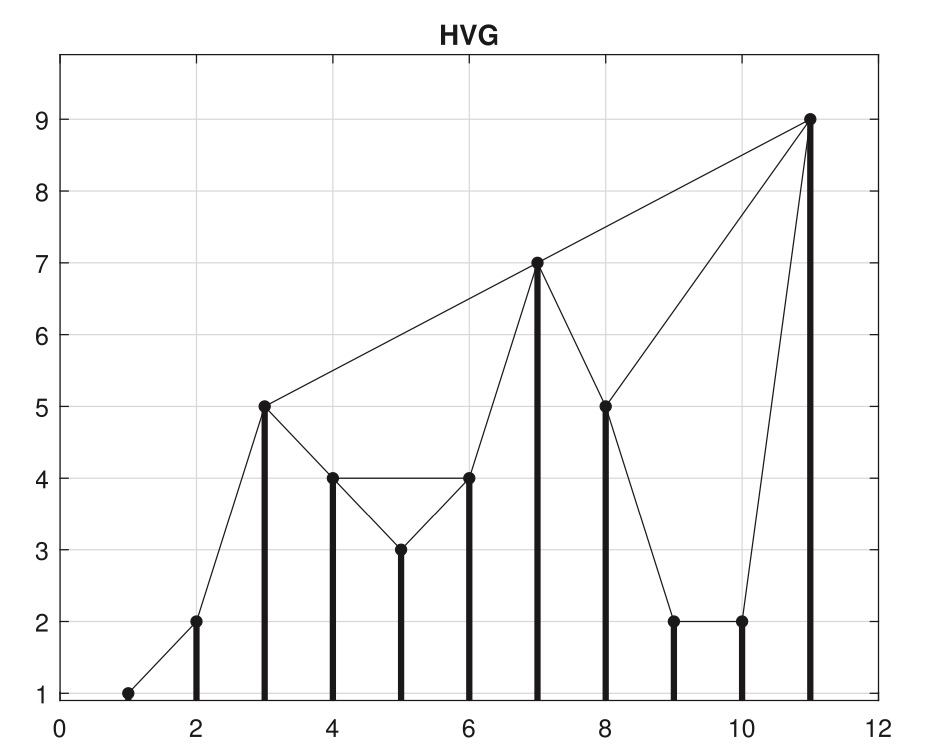
\includegraphics[width=\linewidth]{HVG.jpg}
        \caption{Horizontal visibility graph}
        \label{fig:HVG_example}
    \end{subfigure}
    \caption{Example of NVG and HVG for a time series signal \cite{china_HVG}}
    \label{fig:VG_example}
\end{figure}





\subsection{\textbf{Image Visibility Graphs}}
\subsubsection{INVG: Image natural visibility graph}
\subsubsection{IHVG: Image Horizontal visibility graph}
\subsubsection{Feature extraction }
discuss about local and global features



\section{Feature selection}
This section will discuss the various features that we can choose for our final feature vector; firstly, we discuss each component individually and then demonstrate the final feature vector.


\subsubsection{\textbf{Image, reversed-image}}
As we showed before, the nature of the IVG and HVG definition behaves differently about the local maxima, so taking into account this fact, we calculate features for the original image and reverse image, which is obtained by replacing each pixel value with the maximum pixels value subtracted by the current pixel value.
Figure \ref{fig:original_reversed_texture} shows an example of a texture and its reverse.

\begin{figure}[tbh]
    \centering
    \begin{subfigure}{0.24\textwidth}
        \centering
        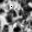
\includegraphics[width=0.55\linewidth]{origianl_fibrosis.png}
        \caption{Original image}
        \label{fig:original_texture}
    \end{subfigure}
    \hfill
    \begin{subfigure}{0.24\textwidth}
        \centering
        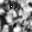
\includegraphics[width=0.55\linewidth]{reversed_fibrosis.png}
        \caption{Reversed image}
        \label{fig:reversed_texture}
    \end{subfigure}
    \caption{original and reversed image of a Fibrosis texture}
    \label{fig:original_reversed_texture}
\end{figure}



\subsubsection{\textbf{IHVG, INVG}}
As we discussed before, we had to choose to define our graphs on images,i.e., natural or horizontal visibility graphs. Our investigation indicates that both of these definitions are useful for describing the textures, and we finally chose features from both of these graph types.
Figure \ref{fig:lattice_nolattice_example} is an artifial $3\times3$ image and INVG is drawn for with Lattice and with No-lattice condition.



\begin{figure}[tbh]
    \centering
    \begin{subfigure}{0.24\textwidth}
        \centering
        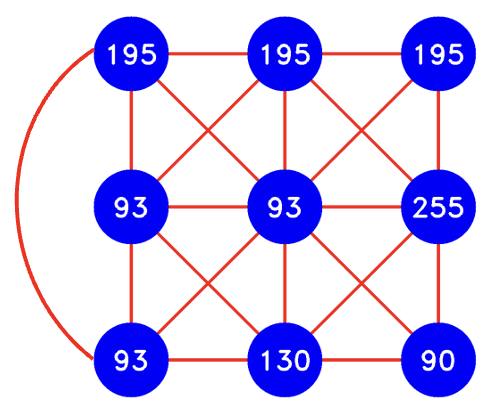
\includegraphics[width=0.55\linewidth]{Lattice_IVG.png}
        \caption{With lattice}
        \label{fig:lattice_example}
    \end{subfigure}
    \hfill
    \begin{subfigure}{0.24\textwidth}
        \centering
        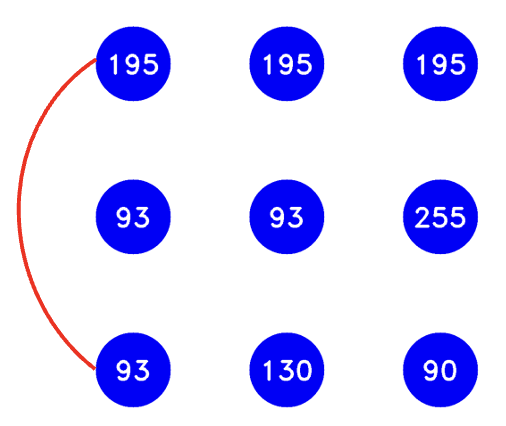
\includegraphics[width=0.55\linewidth]{Nolattice_IVG.png}
        \caption{Without lattice}
        \label{fig:nolattice_example}
    \end{subfigure}
    \caption{An example of INVG with and without lattice}
    \label{fig:lattice_nolattice_example}
\end{figure}


\subsubsection{\textbf{Lattice, without lattice}}
Based on the definition of a visibility graph, each pixel is connected to all of the neighbor pixels, so for simplicity, we can choose to consider these links or not. If we decided not to consider these links, we would have a visibility graph with no-lattice and vice versa. No-lattice graphs result in a more simple graph representation and a more sparse adjacency matrix.


It is good to mention that we can choose both local and global features for each visibility graph configuration; we implemented local feature extraction with $3\times3$ windows and stride one. Also, for global features, we calculate the degree distribution for the graph and plot the histogram of it, then fit a Weibull distribution to that, which will give us two elements for the feature vector, so each of the visibility graph feature vectors is a 258-dimensional vector which the first 256 element is for local feature extraction, and the rest is for global features.

\subsubsection{\textbf{wavelet}}
The method discussed in \cite{wavelet} is a very innovative approach to defining a graph-based feature vector for a texture. We implement that method with a 2-level bipartite graph, and two levels of image,i.e., only one subsampling from $32\times32$ texture resulting in a $16\times16$ texture, and with Meyer kernel for graph wavelet filter with a filter length of 24.
This method for each texture results in a 48-dimensional feature vector, and we can calculate it for both original textures and reversed textures, as discussed before. 


\subsubsection*{\textbf{Final choice}}
Suppose we concatenate all of the possible choices for the final feature vector. In that case, it will give us a 2160-dimensional feature vector for a $32\times32$ texture image which is not desired and can cause overfitting of the model and harder convergence for the classifier. So we sort each feature vector component based on their part in total varience of data,this job done by the same strategy of primary component analysis. Before that, we have to make the feature vectors zero-mean and unit length (due to zero-mean, this has the same effect of making the data unit variance) to make all data have the same scale. Otherwise, we do not get correct result. Also, an essential consideration in machine learning theory is to only perform PCA and data-preprocess (zero-mean and unit length) on Train data, which will be discussed later and not on the full dataset.
Figure \ref{fig: PCA1} shows a pie chart that indicates part of the total variance of data for each possible feature vector component. We should mention that sum of the variance of all global feature extraction methods for visibility graph components was only 1.3\% of all variance. Hence, we decided to remove them from the final feature vector for training our classifier. We concatenate all possible feature vector components except three\: Image-IVG-Nolattice, Reversed-Image-HVG-Nolattice, and Reversed-Image-IVG-Nolattice, which will give us a 1376-dimensional feature vector for each texture.

\begin{figure}[tbh]
  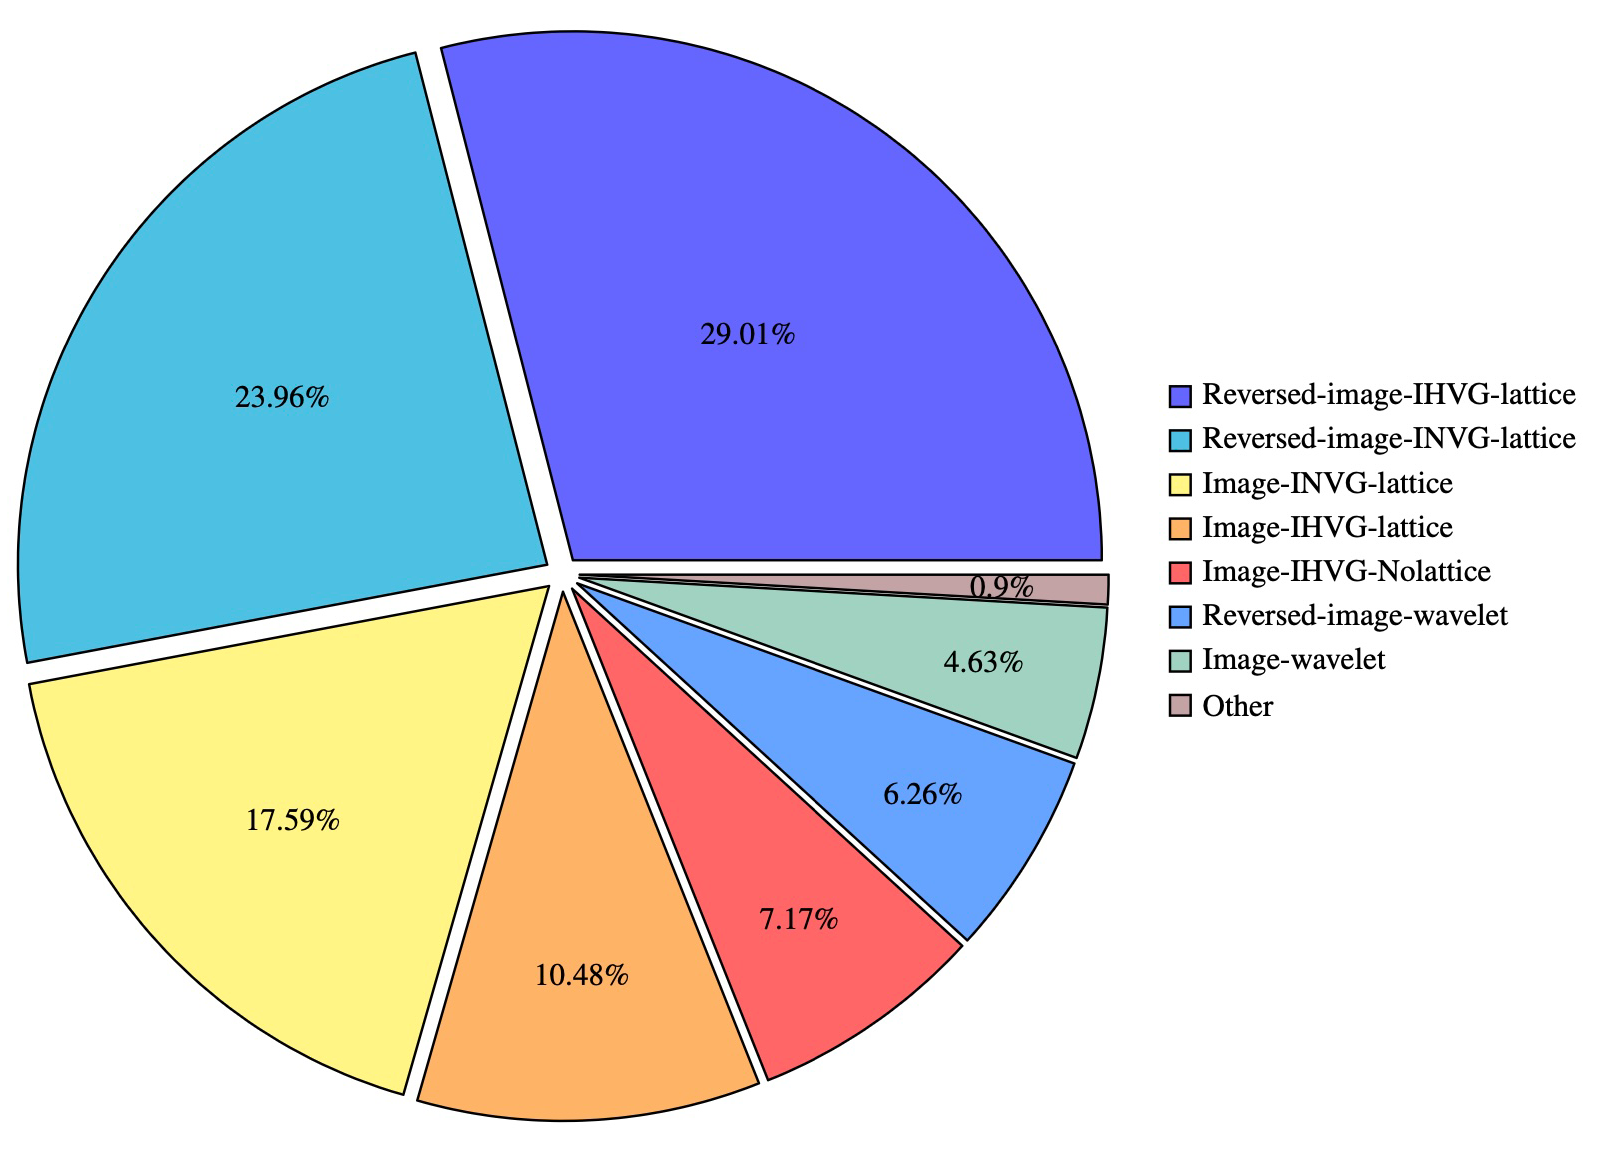
\includegraphics[width=1\linewidth]{PCA_piechart.png}
      \caption{Importance of each feature vector component based on the variance of all data}
  \label{fig: PCA1}
\end{figure}



%\pie[explode=0.1,text = pin ]
%    {
%	29.01/Reversed-image-IHVG-lattice,
%    23.96/Reversed-image-INVG-lattice,
%    17.59/Image-INVG-lattice,
%    10.48/Image-IHVG-lattice,
%    7.17/Image-IHVG-Nolattice,
%    6.26/Reversed-image-wavelet,
%    4.63/Image-wavelet,
%    0.9/Other}
%   \label{pie: PCA1}
%\end{tikzpicture}


\section{Experiment}
\subsection{\textbf{Dataset}}
\subsection{\textbf{preprocessing \& Classifier}}

Due to unbalanced data distribution between various classes, we used five-fold stratified cross-validation. For each fold, we make train data zero-mean with a unit length. Then, with the aim of the primary component analysis, we only chose features that make up 95.83\% of all data variation. Before PCA feature vector length was 1376, and after PCA was 561. We have to use the same transform applied to train data for data preprocess and PCA for test data in each fold. After this transformation, the mean of the test data is not necessarily zero.

For the classifier, we used support vector machine, SVM, with a gaussian kernel and one-vs-other strategy for our multiple class problem. Also, to address the imbalanced distribution of data between classes, we used weighted SVM to solve this issue,i.e., for the class with the least data, the SVM weight is the largest.





\subsection{\textbf{Results and comparison}}

After extracting features and preprocessing the data we trained an SVM classifier as discussed before and we get an overall accuracy of 95.22\%, in each fold of cross-validation we concatenate the prediction for test partition and the overall accuracy is from concatenation of all these partitions.


Table  \ref{cm:CM} shows confusion matrix for final classifier.



\begin{table}[tbh]
\caption{Table of Confusion Matrix for classification}
\label{cm:CM}
\small
\centering
%\begin{tabular}{@{}|lllllc|@{}}
%\begin{tabular}{c|c|*{8}{c|}}
%\begin{tabular}{@{}|lllllc|@{}}
\begin{tabular}{@{}lllllllll@{}}
&& \multicolumn{3}{c}{Predicted label}\\
\toprule
 & H & GG & M & E & F \\ \midrule
 
H (Healthy) & 734 & 25 & 28 & 5 & 3 \\ 
GG (Ground galss) & 44 & 218 & 9 & 1 & 22 \\ 
M (Micronodules) & 80 & 5 & 1052 & 1 & 23 \\ 
E (Emphysema) & 53 & 5 & 7 & 114 & 4 \\ 
F (Fibrosis) & 8 & 29 & 12 & 2 & 484 \\ \bottomrule

\end{tabular}
\end{table}




\begin{table}[tbh]
\caption{Results}
\label{cm:result}
\small
\centering
\begin{tabular}{@{}lllllllll@{}}
\toprule
&accuracy&recall  &precision & TN-rate &   AUC   &  F1-score \\ \midrule

H & 91.71\% & 92.33\% & 79.87\% & 91.49\% & 91.91\% & 85.65\% \\ 
GG & 95.28\% & 74.15\% & 77.3\% & 97.61\% & 85.88\% & 75.69\% \\ 
M & 94.44\% & 90.61\% & 94.95\% & 96.9\% & 93.76\% & 92.73\% \\ 
E & 97.37\% & 62.3\% & 92.68\% & 99.68\% & 80.99\% & 74.51\% \\ 
F & 96.53\% & 90.47\% & 90.3\% & 97.86\% & 94.17\% & 90.38\% \\   \bottomrule
\vspace{-0.25cm} \\ 
Overal & 87.67\% & 87.67\% & 87.67\% & 96.92\% & - & 87.67\% \\ 
\vspace{-0.3cm} \\ 
\bottomrule

\end{tabular}
\end{table}







\vspace{1cm}
\section{Conclusions}
\vspace{1cm}





%\begin{thebibliography}{00}
%\bibitem{b1}
%Laifan Pei, Zhaohui Li, and Jie Liu , "Texture classification based on image (natural and horizontal) visibility graph constructing methods", Chaos 31, 013128 (2021) https://doi.org/10.1063/5.0036933
%\bibitem{b2}
%Qiao, Y-L, Zhao, Y, Song, C-Y, Zhang, K-G, Xiang, X-Z. Graph wavelet transform for image texture classification. IET Image Process. 2021; 15: 2372– 2383. https://doi.org/10.1049/ipr2.12220
%\end{thebibliography}

\bibliographystyle{IEEEtran}
\bibliography{allref.bib}



\vspace{12pt}

\end{document}












